\section{Deployment Planning}
\label{sec:deployment_planning}

Planning for new goals.

A goal is deployable if all its context conditions and dependencies are satisfiable. If a goal is satisfiable there is a deployment plan that is able to satisfy this goal. A deployment plan consist of a set of artifacts that form a closure in the dependency graph and all nodes has context conditions satisfiable.

\begin{figure}[!htb]
  \centering
  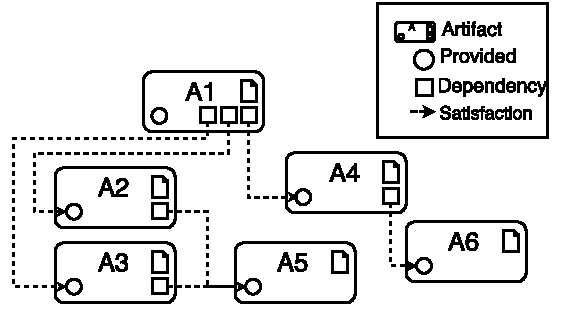
\includegraphics[width=.6\linewidth]{dependency_graph}
  \caption{Dependency Graph}
  \label{fig:dependency_graph}
\end{figure}

\begin{algorithm}
 \KwIn{A goal}
 \KwResult{DeploymentPlan plan}
 \caption{doPlanDeployment(Goal goal)}
 \label{alg:deployment_plan}

 List [] artifacts $\leftarrow$ getArtifactsThatProvide(goal)\;
 \ForEach{Artifact artifact in artifacts}{
   	Boolean contextSatisfaction $\leftarrow$ isSatisfied(artifact.contextConditions)\;
    \If{contextSatisfaction}{
      DeploymentPlan plan $\leftarrow$ new DeploymentPlan()\;
      \ForEach{Goal dependency in artifact.dependencies}{
          DeploymentPlan subPlan  $\leftarrow$ doPlanDeployment(dependency)\;
          \If{!dependencySatisfaction == NULL}{
            \Return{NULL}
          }\Else{
            plan.add(subPlan);
          }
      }
      \Return{plan}
    }\Else{
      \Return{NULL}
    }
  }
\end{algorithm}
